\documentclass[12pt]{article}
\usepackage{geometry}
\usepackage[utf8]{inputenc}
\geometry{a4paper, total={170mm,257mm}, left=2cm, right=2cm, top=2cm, bottom=2cm}
\usepackage{xcolor}
\usepackage[	colorlinks=true, 	urlcolor=blue, linkcolor=green ]{hyperref}
\usepackage{graphicx}
\graphicspath{ {./home/patrick/Desktop/DA_Jehle_Krismer_Motor/DA_Anfrage/DA_Anfrage_Krismer_Jehle_4BHEL_v2/} }
\title{\textbf{\LARGE{DA-Antrag}}}
\author{5BHEL - - Simon Jehle, Patrick Krismer}

\begin{document}
	\maketitle 
***\\
Wir haben ein  Github Repository für die Diplomarbeit:\\
 	\url{https://github.com/Krismoeoeoe/Diploma_Elektromotorpruefstand_Jehle_Krismer}. \\
	Da sind alle Bilder vom Pruefstand, die vorherige Diplomarbeit (als PDFs), Antragsversionen, Datenblätter, Schmierzettel und  Linnks drauf.\\
\begin{itemize}



\begin{figure}
	\centering
	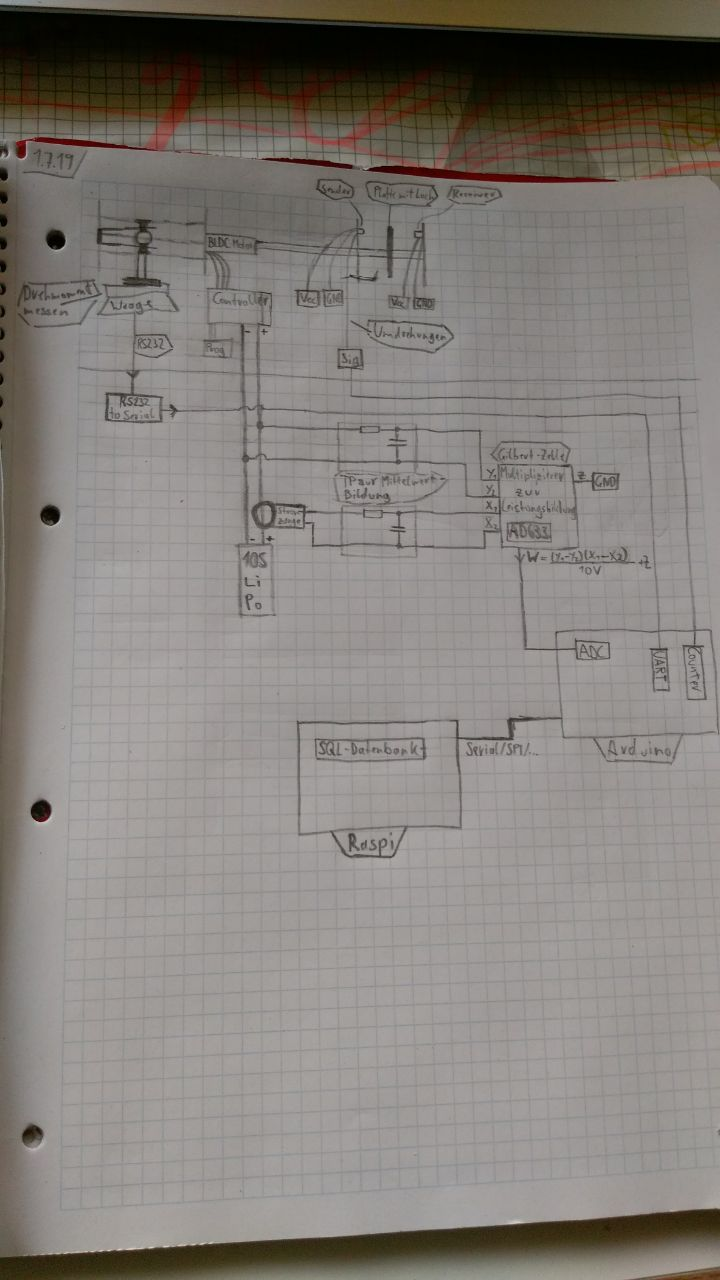
\includegraphics[scale=2.2]{Pruefstandplan_1.png}\\
	\textit{ Pruefstandplan 1 } konstruiert von Simon Jehle (supertyp)
\end{figure}




\subsection*{Ausgangslage }
%\item[•]ALT:\\
%Für einen Elektromotorprüfstand in der HTL, von FISCHER Christian, DI (FS), wird eine möglichst fehlerfreie Steuerung gebaut. Bei dieser Steuerung sollen die Wirkungsgradmessserien weitgehend automatisiert sein, die Messergebnisse in einer Datenbank gespeichert und grafisch dargestellt werden.  \\
%Gemessen werden die Wirkungsgrade eines 'Dualsky XM6360EA-10' bürstenlosen-Elektromotors bei verschiedenen Drehzahlen und Belastungsstufen. 
%Diese Belastungsstufen werden durch eine \textbf{Magnetbremse} simuliert. \\ 
%Die Bremse basiert auf dem Prinzip der magnetischen Hysterese. \\
%Der Wirkungsgrad des Motors ist P-out / P-in\\

\item[•]NEU:\\
\textit{Für einen Elektromotorprüfstand in der HTL, von FISCHER Christian, DI wird eine möglichst fehlerfreie Steuerung gebaut. 
Gemessen werden die Wirkungsgrade eines 'Dualsky XM6360EA-10' bürstenlosen-Elektromotors bei verschiedenen Drehzahlen und Belastungsstufen. 
Die Messergebnisse in einer Datenbank gespeichert und grafisch dargestellt.
Diese Belastungsstufen werden durch eine Magnetbremse, basierend auf dem Prinzip der magnetischen Hysterese simuliert.\\
Des NEUE: 454 Zeichen - - immer noch zu lang :( }\\\\

\item[•]NEUNEU:\\
Einen Elektromotorprüfstand in der HTL, von FISCHER Christian DI (FS), misst  die Wirkungsgrade eines bürstenlosen Elektromotors bei verschiedenen Drehzahlen und Belastungsstufen. \\
Die Belastung wird mittels einer Wirbelstrombremse simuliert. \\Der Motor wird durch zwei Netzgeräten versorgt, die Messungen sind durch Schwankungen in der Versorgung unbrauchbar. \\
Es gibt keine Sicherung bei Überlastung. \\
\textit{\textbf{Fuckin' 400 Wörter genau}}

%\item[•] Durch eine Tiefpassschaltung wird eine Mittelwertbildung an der Spannungsversorgung erreicht, die sonst durch ihre nichtlinearität das Messergebnis vefälscht\\

%\textit{// Sollen wir jetzt für die 110 A  LithiumBatterien oder doch netzgeräte nehmen?}\\

%\textit{//Die Automatische Verstellung des Bremssattels lassen wir im Antrag weg.\\
%//Motorstrom und -Temperaturschutz lassen wir im Antrag weg.\\ 
%//Falls noch Zeit bleibt, machen wir das dazu. (Falls keine Zeit -> habens es nicht im Antrag erwähnt)\\}

 %\begin{figure}
% \includegraphics[scale=1]{DA_Formeln.png} 
 %\caption{\textit{//Sollen wir die Formeln auch in den DA-Antrag schreiben? Oder gehören die erst dann in die Dokumentation (da müssen wir sie sowieso rein schreiben.)}}
%\end{figure}

\newpage
\subsection*{Zielsetzung:}

Ziel ist es eine Messanlage für einen Motorprüfstand zu bauen, welcher den Wirkungsgrad 
bei verschiedenen Drehzahlen und Belastungen misst. Die Ergebnisse werden von einem Arduino 
verarbeitet und an einen Raspberry Pi geschickt, welcher sie in einer Datenbank speichert.\\\\\\

\item[•]Damit der Elektromotor nicht beschädigt wird schaltet der Raspberry Pi automatisch den Motor aus, sobald seine Belastung bzw. die Eingangsleistung einen kritischen Wert überschreitet.\\\\         %in einen kritischen Bereich kommt

\subsection*{Geplantes Ergebnis:}
Ein funktionierender Motorenprüfstand für DC betriebene Elektromotoren, bei verschiedenen Drehzahlen und Belastungsstufen die Wirkungsgrade erfasst.\\
%Es soll eine möglichst fehlerfreie Wirkungsgradmessung eines Elektromotors möglich sein und die 
Die Messwerte werden von einem Arduino-Mega gemessen und bearbeitet. \\
Die Ergebnisse werden in einer Datenbank auf einem Raspberry-Pi-3-B gespeichert.\\
Die Ergebnisse werden grafisch und numerisch dargestellt.\\
\textit{\textbf{355 Wörter}}\\\\


\subsection*{Rechtlichen Regelungen:}
Es gelten die Rechtlichen Regelungen der HTBLVA Anichstraße.\\\\
Kontaktperson:  FISCHER Christian (FS), DI\\


\newpage
\subsection*{Arbeitsaufwand:}

\underline{\textbf{Simon Jehle, 4BHEL: 180 Stunden}}
\item[•] Zeitplanung
\item[1] Arduino Eingangsleistungsmessung (Motor) 
\item[2] Arduino Leistungsabgabenmessung (Präzisionswaage) 
\item[3] Programmierung der Kommunikation zwischen Raspi und Arduino 
\item[4] Selbstaktuallisierendes Informationsinterface (Gibt Auskunft über aktuelle Messwerte) \\\\
%Zeitplanung, Programmierung Arduino (Datenverarbeitung), Programmierung Raspberry Pi (Datenbank, Messsteuerung)\\
%Kommunikation zwischen den beiden Embedded Systems\\

\underline{\textbf{Patrick Krismer, 4BHEL: 180 Stunden }}
\item[•] Zeitplanung
\item[1] Motoransteuerung (verschiedene Drehzahlen, etc. )  
\item[2] Wirbelstrombremsensteuerung + Featback (Aktuelle Belastungsstufe)  
\item[3] Raspberry Pi (Datenbank, etc. ) 
\item[4] Automatisierte Notabschaltnug des Motor 
\item[5] Dokumentation, Präsentation
%Leistungsberechnungen, Messschaltungen (Tiefpassschaltung (mit Reset, Entladung des Kondensators)), Kommunikation Arduino-Waage\\\\


\subsection*{Meilensteine:} 
\begin{tabular}{| l | l |}
\hline
\textbf{1. Meilenstein: } & \textbf{24. September 2019} \\ \hline & \\
Jehle & Arduino Eingangsleistungsmessung (Motor) \\ & \\

Krismer & Motoransteuerung (verschiedene Drehzahlen, etc. ) \\ & \\ \hline  					%Leistungsberechnungen, Filter-Tiefpassschaltung 



\textbf{2. Meilenstein: } & \textbf{04. November  2019} \\ \hline & \\
 Jehle &  Arduino Leistungsabgabenmessung (Präzisionswaage) \\ & \\
 
Krismer & Wirbelstrombremsensteuerung \\ & \\ &  + Featback (Aktuelle Belastungsstufe)  \\ & \\ \hline 


\textbf{3. Meilenstein: } & \textbf{16. Dezember 2019} \\ \hline & \\
Jehle & Programmierung der Kommunikation zwischen \\
           & Raspi und Arduino\\ & \\
           
Krismer &  Raspberry Pi (Datenbank, etc. ) \\ & \\
%Notausschaltung mittels Komparator 						%Schaltungsaufbau Testen 


\textbf{4. Meilenstein: } & \textbf{24. Februar 2020} \\ \hline & \\
Jehle & Selbstaktuallisierendes Informationsinterface \\ & \\ & (Gibt Auskunft über aktuelle Messwerte)\\ & \\

Krismer &  Automatisierte Notabschaltnug des Motor \\   & \\ \hline 


\textbf{5. Meilenstein: } & \textbf{23. März 2020} \\ \hline & \\
Jehle & \textit{Raspberry Pi, Automatische Messung }\\ & \\
Krismer & Dokumentation fertig, Präsentation fertig\\ & \\ \hline
\end{tabular} 






\newpage
\subsection*{Voraussichtliches Equippment}
 \item[-]Arduino Leonardo / Mega (wegen mehr Interrupts als UNO (ATMega32u4)) 
 \item[-]Raspberry Pi (Ziemlich egal, muss nit Heizer Version 4 sein) 
 \item[-]SD Karte für RPi (Plus Sachen für Verbindung zu vllt. Auswertungs-PC) 
 \item[-]AD633 Multiplizierer 
 \item[-]CP1100 Stromzange (müsste FS noch haben),  
 \item[-]Bauteile für TP (Widerstände, Kondensatoren, Transistoren),  
 \item[-]10S LiPo (Fischer hat von 10S LiPo geredet),  
 \item[-]IGBT oder Solid-State-Relais (LiPo zu Controller Verbindung),  
 \item[-]RS232 zu Serial Converter   (von "Kern Präzisionswaage 440-51N" zum  Arduino zum Drehmoment messen), 
 \item[-] 5V Netzteil, 
 \item[-] Komparator (Notausschaltung), 
 \item[-]Kabel, Verbindungen, Widerstände (Pulldown), usw. 
  \item[-]Litium Ionen Akuumulatoren
  
  
\subsection*{Verwendete Embedded Systems:}
\textit{Also, die Messung startet sobald Arduino und Raspi gestartet sind und der Motor Strom hat. \\
				Wenn die Grafik dann generiert ist, soll die Messung dann aufhören oder noch weiter laufen für eine weitere Messung?}
\item[-]\textbf{Arduino (-Mega):}\\
verarbeitet die Messergebnisse der Sensoren bzw. direkt am Arduino anliegende Signale \\
und gibt sie dann an den Raspberry Pi weiter.\\
Aus der Datenbank wird anschließend eine Grafik erstellt, die den Wirkungsgrad bei verschiedenen Drehzahlen darstellt.\\\\ 

\item[-]\textbf{Raspberry Pi (-3-B):}\\
Er betreibt eine Datenbank in der die Messergebnisse gespeichert werden.\\


\end{itemize}
\end{document}